\documentclass[letterpaper]{article}
\usepackage[utf8]{inputenc}				% use Unicode
\usepackage{hyperref}
\setlength\parindent{0pt}				% no indentation at start of paragraph
\usepackage{multicol}
\usepackage{graphicx}
\usepackage{float}
\graphicspath{{./figures/}}

\newcommand{\p}{\vspace{1em}\par}		% macro to start new paragraph

\author{David De Lille}
\title{Offensive Computer Security: Summary 2}

\begin{document}
\maketitle

\section{Intro to CPU and registers}
\subsection{Registers}

\begin{center}
\begin{tabular}{cccc}
64-bit register & lower 32-bit & lower 16 bit & lower 8 bit\\
\hline
rax & eax & ax & al\\
rbx & ebx & bx & bl\\
rcx & ecx & cx & cl\\
rdx & edx & dx & dl\\
rsi & esi & si & sil\\
rdi & edi & di & dil\\
rbp & ebp & bp & bpl\\
rsp & esp & sp & spl\\
r8 & r8d & r8w & r8b\\
r9 & r9d & r9w & r9b\\
r10 & r10d & r10w & r10b\\
r11 & r11d & r11w & r11b\\
r12 & r12d & r12w & r12b\\
r13 & r13d & r13w & r13b\\
r14 & r14d & r14w & r14b\\
r15 & r15d & r15w & r15b
\end{tabular}
\end{center}

\begin{multicols}{2}
\begin{itemize}
\item eax: accumulator (return value)
\item ebx: base
\item ecx: count
\item edx: data
\item ebp: base pointer
\item esi: source index
\item edi: destination index
\item esp: stack pointer
\item eip: instruction pointer
\end{itemize}
\end{multicols}
%64-bit registers are similar, but their names start with "r".

\begin{figure}[H]
\centering
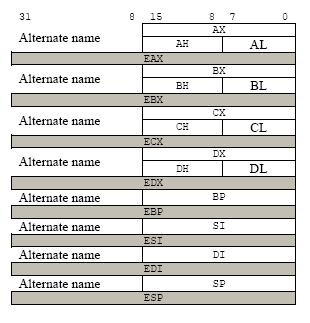
\includegraphics[scale=0.70]{registers.png}
\end{figure}


\section{Why learn C?}
\begin{itemize}
\item one of the most widely used programming languages
\item other popular languages borrow from it
\item used in everything (OS, embedded systems, drivers, libraries, other prog. languages)
\end{itemize}

\section{Strings}
\subsection{String types}
A \emph{string} is an array of characters up to and including the terminating null character. \emph{Length} = the number of characters including the null character. \emph{Count} = number of elements in the array. \emph{Size} = the number of bytes allocated to the array. Size of a string depends on the size of the characters and can be larger than the length.

\p Character types:
\begin{itemize}
\item \mbox{[signed/unsigned] char}
\item \mbox{[signed/unsigned] wchar\_t (not meant to be signed/unsigned)}
\end{itemize}

wchar\_t is an integer type that can represent the largest character set among the supported locales. On Windows, it uses UTF-16 (2 bytes per character). On Linux, it uses UTF-32 (4 bytes per character).

\subsection{String functions}
Length/Size functions:
\begin{itemize}
\item strlen (run time)
\item sizeof (compile time)
\item wcslen (for wide characters)
\end{itemize}

Copying:
\begin{itemize}
\item \href{http://www.cplusplus.com/reference/cstring/memcpy/}{memcpy}: Copy block of memory 
\item \href{http://www.cplusplus.com/reference/cstring/memmove/}{memmove}: Move block of memory 
\item \href{http://www.cplusplus.com/reference/cstring/strcpy/}{strcpy}: Copy string (unbounded)
\item \href{http://www.cplusplus.com/reference/cstring/strncpy/}{strncpy}: Copy characters from string 
\item \href{https://msdn.microsoft.com/en-us/library/td1esda9.aspx}{strcpy\_s}: (A windows function, not C99/C11)
\item POSIX function (not C99/C11): strdup
\item Windows functions (not C99/C11): \href{https://msdn.microsoft.com/en-us/library/kk6xf663.aspx}{wcscpy}, \href{https://msdn.microsoft.com/en-us/library/td1esda9.aspx}{wcscpy\_s}, \href{https://msdn.microsoft.com/en-us/library/kk6xf663.aspx}{\_mbscpy}, \href{https://msdn.microsoft.com/en-us/library/td1esda9.aspx}{\_mbscpy\_s}
\end{itemize}

Concatenation:
\begin{itemize}
\item \href{http://www.cplusplus.com/reference/cstring/strcat/}{strcat}: Concatenate strings
\item \href{http://www.cplusplus.com/reference/cstring/strncat/}{strncat}: Append characters from string
\item \href{http://www.cplusplus.com/reference/cstdio/sprintf/}{sprintf}: Format strings (also copying)
\item \href{http://www.cplusplus.com/reference/cstdio/snprintf/}{snprintf}: Format strings (also copying)
\end{itemize}

\subsection{Common errors/vulnerabilities}
\subsection{Improperly bounded string copies}
The functions gets (cannot be used safely) and strcpy (can be used safely) are deprecated. However, misuse of their replacements can also be unsafe: strncpy, memmove, memcpy, sprintf, snprintf. Example on slide 24-27.

\subsection{Off-by-one errors}
This involves reading/writing outside the bounds on an array. Example on slide 29.

\subsection{String truncation}
Data is lost when a too large strings is put (safely) into too small of a destination. This can lead to errors in the application logic.

\subsection{Null termination errors}
When a string isn't properly null terminated. The functions strncpy and strncat don't null terminate.

\subsection{Preventing errors/Mitigations}
\begin{itemize}
\item use \href{http://websec.github.io/unicode-security-guide/character-transformations/}{encoding best practices}
\item use safe function correctly
\item use a unified model for handling strings (see slide 70)
\item use stack cookies (more details in further lectures)
\end{itemize}

\section{Pointers}
\subsection{Asterisk operator: *}
When used for declaring, it instantiates a variable pointing to an object of the given type.

\p When used an a unary operator, it denotes indirection. If this operator doesn't point to an object or function, the behaviour is undefined. Dereferencing NULL is a vulnerability if it is a memory-mappable address.

\subsection{Ampersand operator: \&}
This operator shows the actual data stored in a pointer. It is used to get the address of an object.

\subsection{Member-of operator: -$>$ }
This deferences a structure and accesses a member of that structure.

\subsection{Array indexing: x[y]}
This calculates the address based on the address of x and the value of y.

\subsection{Function pointers}
This type of pointer points to executable code in memory. This can be very dangerous if it can be made to point to malicious code. Example on slide 42. Notice the use of register al on slide 45, line 14 in the Assembly code.

\subsection{Global Offset Table (GOT)}
This is the section of an ELF-file (Executable and Linking Format) that holds absolute addresses for all accessed global variables, and is essential for dynamically linked libraries. This is used to make the code position-independent. Executables on Windows use a similar technique for using libraries, but only the Linux version is exploitable.

\p Before a library function is used, the GOT points to the Run Time Linker (RTL). When the function is called, the RTL finds the actual address and writes it into the GOT. Any subsequent calls use the function's address directly, without involving the RTL.

\p The GOT is located at a fixed address in every ELF, and it is not write-protected because the RTL needs to be able to change it. If the GOT can be overwritten by an attacker, it can be used to redirect an existing function to malicious shellcode.

\subsection{.ctors and .dtors section}
This is a section added by the GCC compiler, that contains the destructor function pointers. These function pointers will be executed after main exits. The function pointers in the related .ctors section are executed before main, and are therefore never targeted. 

\subsection{Find-the-bug exercises}
Slide 43-45: The code on the left allocates memory and truncates the address by storing it in a char variable, which is only 1 byte instead of the required 4 or 8 bytes.

\p Slide 46: ...

\p Slide 52: The first if-structure checks that a member function isn't NULL. After that, the second one checks that s isn't NULL. If s was indeed NULL, this would mean that the first if-structure has dereferenced s (which is NULL).

\p Slide 53: The else-clause of the if-structure is only executed if subnet is NULL, but then it calls a member function of subnet (subnet->Name()), which would be dereferencing NULL.

\p Slide 54: (I think the "mp" seen on the slide should be "tmp".) I think the bug is in the dereferencing of tmp, without checking that it might be NULL. Another possibility is that the member mListNodePrev might be NULL, which would cause a NULL-derefence later on.

\section{Dynamic memory management}
\subsection{C memory management}
\subsubsection{C99 memory allocation functions (heap)}
\begin{itemize}
\item malloc
\item alligned\_alloc (see below)
\item realloc: change the size of memory
\item calloc: allocates and sets to 0
\end{itemize}

\subsubsection{Alignment}
This is a restriction on the memory address of certain objects in older systems. Objects have to lie neatly in aligned byte slots. Attempts to use misaligned data would result in a bus error and terminate the program. Modern systems are able to handle it correctly (but slower). This can be important for exploitation.

\subsubsection{Alloca}
This is a function that uses the stack for dynamic memory  allocation. It isn't part of the C99 standard. Obviously this can cause stack overflows.

\subsection{Common errors}
\subsubsection{Initialisation Errors}
Not properly initialising memory. Malloc and free do not zero out memory.

\subsubsection{Failure to check return values}
Assume that the function will succeed can result in edge-case bugs. Malloc will return NULL if there is not enough free heap memory.

\subsubsection{Using Freed memory}
Unless all pointers have been NULLed or invalidated, it's still possible to access the freed memory. Example on slide 60-61. This leads to a vulnerability (see next summary).

\subsubsection{Multiple frees on same memory}
This is usually caused by careless copy-pasting or sloppy error-handling. It can result in a corrupted heap memory manager, segfaults, vulnerabilities, or memory leaks.

\subsubsection{Memory Leaks}
A memory leak happens when a program fails to free dynamically allocated memory after it has been used. The result is that this memory becomes unavailable to the program or the rest of the system, leading to memory exhaustion. If an attacker can exploit memory leaks, it can be used for an DOS attack.

\subsubsection{Dereferencing a NULL pointer}
A null-pointer dereference takes place when a pointer with a value of NULL is used as though it pointed to a valid memory area. If an attacker can intentionally trigger a null pointer dereference, the attacker might be able to use the resulting exception to bypass security logic or to cause the application to reveal debugging information that will be valuable in planning subsequent attacks.

\subsection{Memory allocator}
(see next summary)

\subsection{Mitigations}
\begin{itemize}
\item set pointers to NULL after freeing them
\item use ASLR (see later)
\item testing
\end{itemize}

\section{Required reading: HAOE 0x260 up to 0x280}
I'll just briefly state what each subchapter talks about, since it's mostly C basics.
\subsection*{0x261 Strings}
Strings. GCC -o flag. NULL terminators. The stack stores return addresses when calling functions.
\subsection*{0x262 Signed, Unsigned, Long, and Short}
Numerical values are signed by default. Two's complement. Use sizeof() to find the actual size for that architecture. 
\subsection*{0x263 Pointers}
Use pointers instead of copying large amounts of data. Asterisk and ampersand operators.
\subsection*{0x264 Format Strings}
Format string = character string with escape characters to insert variables in a certain format. Some format parameters are listed.
\subsection*{0x265 Typecasting}
Typecasting = temporarily change a variable's data type. Void pointer. Compiler is the only thing that cares about data types.
\subsection*{0x266 Command-Line Arguments}
Argc and argv. argv[0] = name of binary. Too few program arguments can result in a SEGFAULT.
\subsection*{0x267 Variable Scoping}
Contex. Local and global variables. Stack frames. Static variables.
\subsection*{0x270 Memory Segmentation}
Five segments: text (code), data (initialised global/static vars), bss (uninitialised global/static vars), heap (dynamic memory), and stack (local variables and stack frames). Stack abstract data structure. Frame pointer or local base pointer. Figure of a stack frame (p73). Relative location of the 5 segments (Figure p75).  
\subsection*{0x271 Memory Segments in C}
Which variables get stored in which segment.
\subsection*{0x272 Using the Heap}
malloc() and free().
\subsection*{0x273 Error-Checked malloc()}
Use a function to avoid duplicated error checks around mallocs.

\section{Other notes}
\begin{itemize}
\item \href{http://gcc.godbolt.org}{Godbolt} is a tool that visualises what C/C++ code corresponds to what Assembly code.
\end{itemize}

\end{document}

